% content of the chapter introduction
\chapter {Introduction}
\label{introduction}
\section{Metaphysics}
\label {metaphysics}
Nature (Real world, Universe) is unique and exists independently of us. The observer who appears in physical
literature is nothing more than figure of speech. `Moon exists even nobody looks at it' and so does electron.
Real word objects behave according to Laws of Nature. Contrary to human laws the Laws of Nature could never be violated.
When we read something like 'this device violates laws of physics' it means usually misunderstanding or clickbait (probably both). Discovering of these laws is the goal of physics. 

To achieve this goal
we build Ideal world and populate it by mathematical models. These models emerge as result of  observations (experiments, measurements, experience), 
their elements appear as ideal images of real objects. Using instruments, 
which may be as simple as measuring tape or lever scaling or as complex as electronic microscope or collider, experimental physics gets facts of Real world.
Theoretical physics constructs and update mathematical models 
on base of these facts.
It should be mentioned that our instruments are part of Real world  and hence described by models\footnote{so a person trying 
to disprove say quantum mechanics would have serious problem since every modern instrument is based actually on quantum 
mechanics.}

    When constructing a model, the following idealization is
   made (see e.g. \cite{Arnold-mt}): 
\begin{itemize}
    \item Events which are  highly probable in Real world become certain in ideal one.
    \item Plausible deductions become proofs.
    \item Some (irrelevant) details disappear.
    \item Approximate results become exact.
\end{itemize}               

This is how abstract notions such as perfectly rigid bodies, incompressible fluids, material points, and so on emerge. 
Even the statement that results of measurement are real numbers is actually idealization: no instrument is able to produce output with infinite number of digits, hence experimental results are always rational numbers.

 When reasonable model is constructed, 
it is investigated and conclusions are mapped back to Real world as predictions which 
should be tested by  experiment. 
If we get  accurate description of reality the model remains {\em reasonable} and can be foundation 
for other models, in particular those describing our instruments, if not it  should be replaced or improved in some way or another.
If the model fails to produce results to be experimentally checked, it simply makes no sense.

Let's assume that we have reasonable (mathematical) model. How can
we obtain correct conclusions from it. 
Purely formal reasoning risks gross errors. 
Particularly dangerous is the temptation to demand precise  definitions for every concept and object in a theory: such definitions often rest on seemingly innocent assumptions 
whose physical meaning is unclear. As a result, one may arrive at impeccably logical conclusions that nonetheless bear no relation to the physical problem at hand.

Here mathematician
and physicist take different paths “The mathematician proves, while the physicist convinces.” \cite{Medvedev}. Mathematician rigorously
and carefully investigates the model as it is formulated.
Physicist may change or abandon the model if it yields 
 incorrect results (contradicting to known experimental facts).
Nature is too complex to be described by one model.
Physicist often uses more than one model simultaneously and change them on the fly 
without warning or use some conditions which were not stated explicitly. 
These tricks irritate mathematicians and confuse engineers. However they are natural parts of 
physicist's way of thinking. 

Contrary to what is said in many (good) books the relations 
among models are not necessary hierarchical. Generally model may be a particular case of another one only in restricted domain. 
For example only system of material points interacting via electromagnetic or (and) gravitational
field constitutes the common subject of classical, relativistic and quantum mechanics and only for such systems classical mechanics may be regarded as special case. Systems with constraints generally can not be described in quantum or relativistic theory.

Formal logic belongs to Ideal world only, on the other hand notions like causality,  likelihood, measurements,
`experimental support' make sense only and in Real world and need 
special care when mapped to Ideal world. 

A lot of paradoxes appear when we mix Real and Ideal world. 
Let us take for example  Hempel's raven paradox: ``observing
of red cow increases the likelihood 
that all ravens are black''. 

Indeed suppose that the statement `All ravens are black' is true.
In the form of an 
implication, this can be expressed as: If something is a raven, then it 
is black. Via contraposition, this statement is equivalent to: If something is 
not black, then it is not a raven. So an observation of, say, red cow supports 
the statement that all ravens are black. This looks very strange but actually is quite
straightforward. In formal logic (Ideal world) there is no such thing as experimental support or
likelihood. Statement may be invalidated by the observation of non black raven, 
but can not be confirmed in any way. So contraposition means simply that the 
statement `raven is found which is not black' is equivalent to 
`something not black is found which is raven'. 

On the other hand common sense (Real world) does not allow statements about 
{\em all} ravens. We should say majority or practically all 
and  contraposition  disappears.

Another good example is Schroedinger's cat. In quantum mechanics the (pure) state of the system is described 
by wave function. Nobody knows exact wave function for an object more complicated than hydrogen atom. 
Surely we can use approximate one, but even in that case preparing of the object in pure state
is rather involved task.  Even if somebody can figure out wave function of cat, how to prepare it
in pure state? May be cool it down to $0^\circ K$? Correlations replace causality in Ideal World.
 Life and death exist in Real World only and have no analogs in Ideal World.

Mathematical problems which required for physical predictions, except in the simplest cases, are so complex that only approximate solutions are possible. 
Often we cannot even verify the validity of the approximations we use,
since this would require exact solutions we cannot obtain. Actually we should 
use some form of perturbation theory ---expansion in series over small parameter(s). 
In most cases the convergence of the series is not proved (and sometimes divergence is proved). 
Another way is numerical approach which of course has its own pitfalls.

\section{Limits are dangerous}
\label{limits}
Limits should be taken with care. A number of theorems describe 
when we can change order of limits and when we can not, how
we can approach to the limit and all that.

Imagine a bucket with small hall at the bottom (in Ideal world),
so we can say that the hole is so small that for all times the bucket remains practically full.
On the other hand we can say that the bucket will be empty if we wait long enough.

Important fact is that two smooth curve may coincide as sets of points, but have
different lengths. Let $ y_n= \sin(n x)/n $ on the  interval $ 0\le x \le 2 \pi $. 
Calculation of length of sinusoidal curve is a simple exercise in elliptic integrals:
\begin{equation}
   \label {sin-length}
   \begin{split}
       l_n=\int_0^{2 \pi}\sqrt{1+\cos^2(nx)}dx\\
       =\int_0^{2 n \pi}\sqrt{1+\cos^2(z)}dz/n\\
       =\int_0^{2 \pi}\sqrt{1+\cos^2(z)}dz\quad \text{does not depend on n}  \\
       =4 \sqrt{2} \int_0^{\pi/2}\sqrt{1-\frac{1}{2} \sin^2(z)}dz\\
       =4 \sqrt{2} E(\frac{1}{\sqrt{2}}) \approx 1.351
   \end{split}
\end{equation}  
and ratio of its length to that of segment is $ \approx 1.22 $ independent of $ n $.
On the other hand maximal distance between the curve and straight segment $ d_n=1/n $ 
vanishes for $ n\rightarrow \infty $.

Contrary to common belief not every properly set problem in
classical mechanics has unique solution. Let's take for example
a (rigid) beam on three (rigid) pillars (see fig.\ref{beam3}).
\begin{figure}[h]
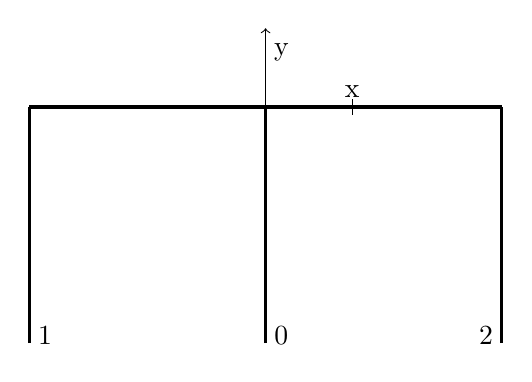
\begin{tikzpicture}
%\draw[thin,dotted] (-3,-3) grid (3,1);
\draw[->] (0,0) -- (0,1);
\node at (0.2,0.7)  {y};
\draw[very thick] (-3,0) -- (3,0);
\draw[very thick] (-3,-3) -- (-3,0);
\draw[very thick] (3,-3) -- (3,0);
\draw[very thick] (0,-3) -- (0,0);
\draw (1.1,-0.1) -- (1.1,0.1);
\node at (1.1,0.2) {x};
\node at (-2.8,-2.9) {1};
\node at (0.2,-2.9) {0};
\node at (2.8,-2.9) {2};
\end{tikzpicture}
\caption{Beam on 3 pillars}
\label {beam3}
\end{figure}
Let the weight of the beam be $W$ and length $2 L$.
Balance of forces gives:
\begin{equation}
        F_0+F_1+F_2=W \label {bf}
\end{equation}
Balance of torques gives:
\begin{equation}
        F_1 L=F_2 L \label {bt}
\end{equation}

   So we have only two equations for three
unknown forces. From the symmetry we can get that $F_1=F_2$. 
(We know that this already from balance of torques.)

{\em First solution}:
All pillars and beam are absolutely rigid. Then
if we pull out the middle pillar nothing will change.
So $F_0=0$ and $F_1=F_2=W/2$.

{\em Second solution}
All pillars and beam are absolutely rigid. Then
we can cat beam at the center and will have two
beams laying on two pillars each.
So $F_0=W/2$ and $F_1=F_2=W/4$.

{\em Third solution}
Beam is absolutely rigid, pillars are very hard springs.
Since beam is horizontal, small change in length is 
equal to all pillars so $F_0=F_1=F_2=w/3$


{\em Fourth solution}
Pillars are rigid, beam is elastic. This case needs
some calculations, well known in elasticity theory
(see e.g \cite {Landau-Lifshitz-7}).
The results is $F_0=5 W/8$ and $F_1=F_2=3 W/16$.

It is clear that all these solutions (and more can be
produced) are limiting cases of standard elasticity 
problem when elasticity coefficients go to infinity.
So generally we can't simply neglect elastic deformations,
we should be more careful.


\section{Units}
\label{units}
Actually to map  physical object into Ideal world of numbers we need some system of units.
What is good about units is that there is plenty of choices.
SI system is the most popular. 
In this system, as described by NIST (National Institute of Standards and Technology, US),
seven base units are defined.
\begin{description}
    \item [time] The second (s) is defined by taking the fixed numerical 
 value of the unperturbed ground-state hyperfine transition 
 frequency of the cesium-133 atom, to be 9,192,631,770 
        when expressed in the unit Hz, which is equal to \unit{ s^{-1}}.
    \item [length] The meter (m) is defined by taking the fixed numerical value of
the speed of light in vacuum c to be 299,792,458 
when expressed in the unit \unit{m.s^{-1}}.
\item [mass] The kilogram (kg) is defined by taking the fixed numerical 
value of the Planck constant h to be $6.62607015 10^{-34}$
when expressed in the unit \unit{J.s}, which is equal to \unit{kg.m^2.s^{-1}}.
\item [electric current] The ampere (A) is defined by taking the fixed numerical value of 
 the elementary charge e to be \num{1.602176634e-19} when expressed in the unit C,
        which is equal to \unit{A.s}.
\item [temperature] The kelvin (K) is defined by taking the fixed numerical value of
    the Boltzmann constant k to be \num{1.380 649e-23} when expressed in the unit \unit{J.K^{-1}}.
\item [amount of substance] Mole (mol) contains exactly \num{6.02214076e23} 
    elementary entities. This number is the fixed numerical value of the Avogadro constant, 
        NA, when expressed in the unit \unit{mol^{-1}}.
\item [luminous intensity] The candela (cd) is defined by taking the fixed numerical 
    value of the luminous efficacy of monochromatic radiation of frequency num{540e12} Hz, Kcd, 
        to be 683 when expressed in the unit \unit{lm.W^{-1}}, which is equal to \unit{cd.sr.W^{-1}}. 
\end{description}
Last three units have no use in theoretical physics and are mentioned for completeness only.

If restricted to length,time and mass all systems of units  differ only 
by scale and hence using of this or that system is a matter of taste. 
For example,to demonstrate good education, one can use 'FFF system' --- Furlong as unit of length (201 m),
Firkin(of water) as unit of mass (41 kg), and Fortnight as unit of time ($ 14\times 86400 s $). 

The situation is more complicated when when we consider electromagnetic phenomena. SI introduces
amper as independent unit which allows to use familiar units for voltage, current and so on.
However the price for that is too high, dimensional permeability of vacuum emerges, components
of electromagnetic field are measured with different units etc. So I shall use Gaussian system,
time is measured in seconds, length in centimeters, and mass in grams. Unit of charge is defined
so that Coulomb low is written as
\[ U= \frac{q_1 q_2}{r} \]
so its dimension is \unit{g^{1/2}.cm^{3/2}.s^{-1}}. 

Anyway, despite of efforts of proponents of SI, a number of external units is popular in practice.
In elementary particle physics energy is mostly measured in electron-volts (\unit{eV}) 
which is equal to  \num{1.602176634e-19} J,
while in
power engineering  in kilowatt-hours (\unit{kW}) equal to \num{3.6e6} J.
Interesting to see that kinetic energy of flying mosquito is approximately 4 \unit{TeV}, and total electric energy 
produced in US in 2022 is approximately \num{1.6e19} J, which correspond to approximately 200 \unit{kg}
according to $ E=m c^2 $ formula.

\section{Numerical methods}
\label{numerical-methods}
TBD
